\begin{figure}[t]
    \centering
    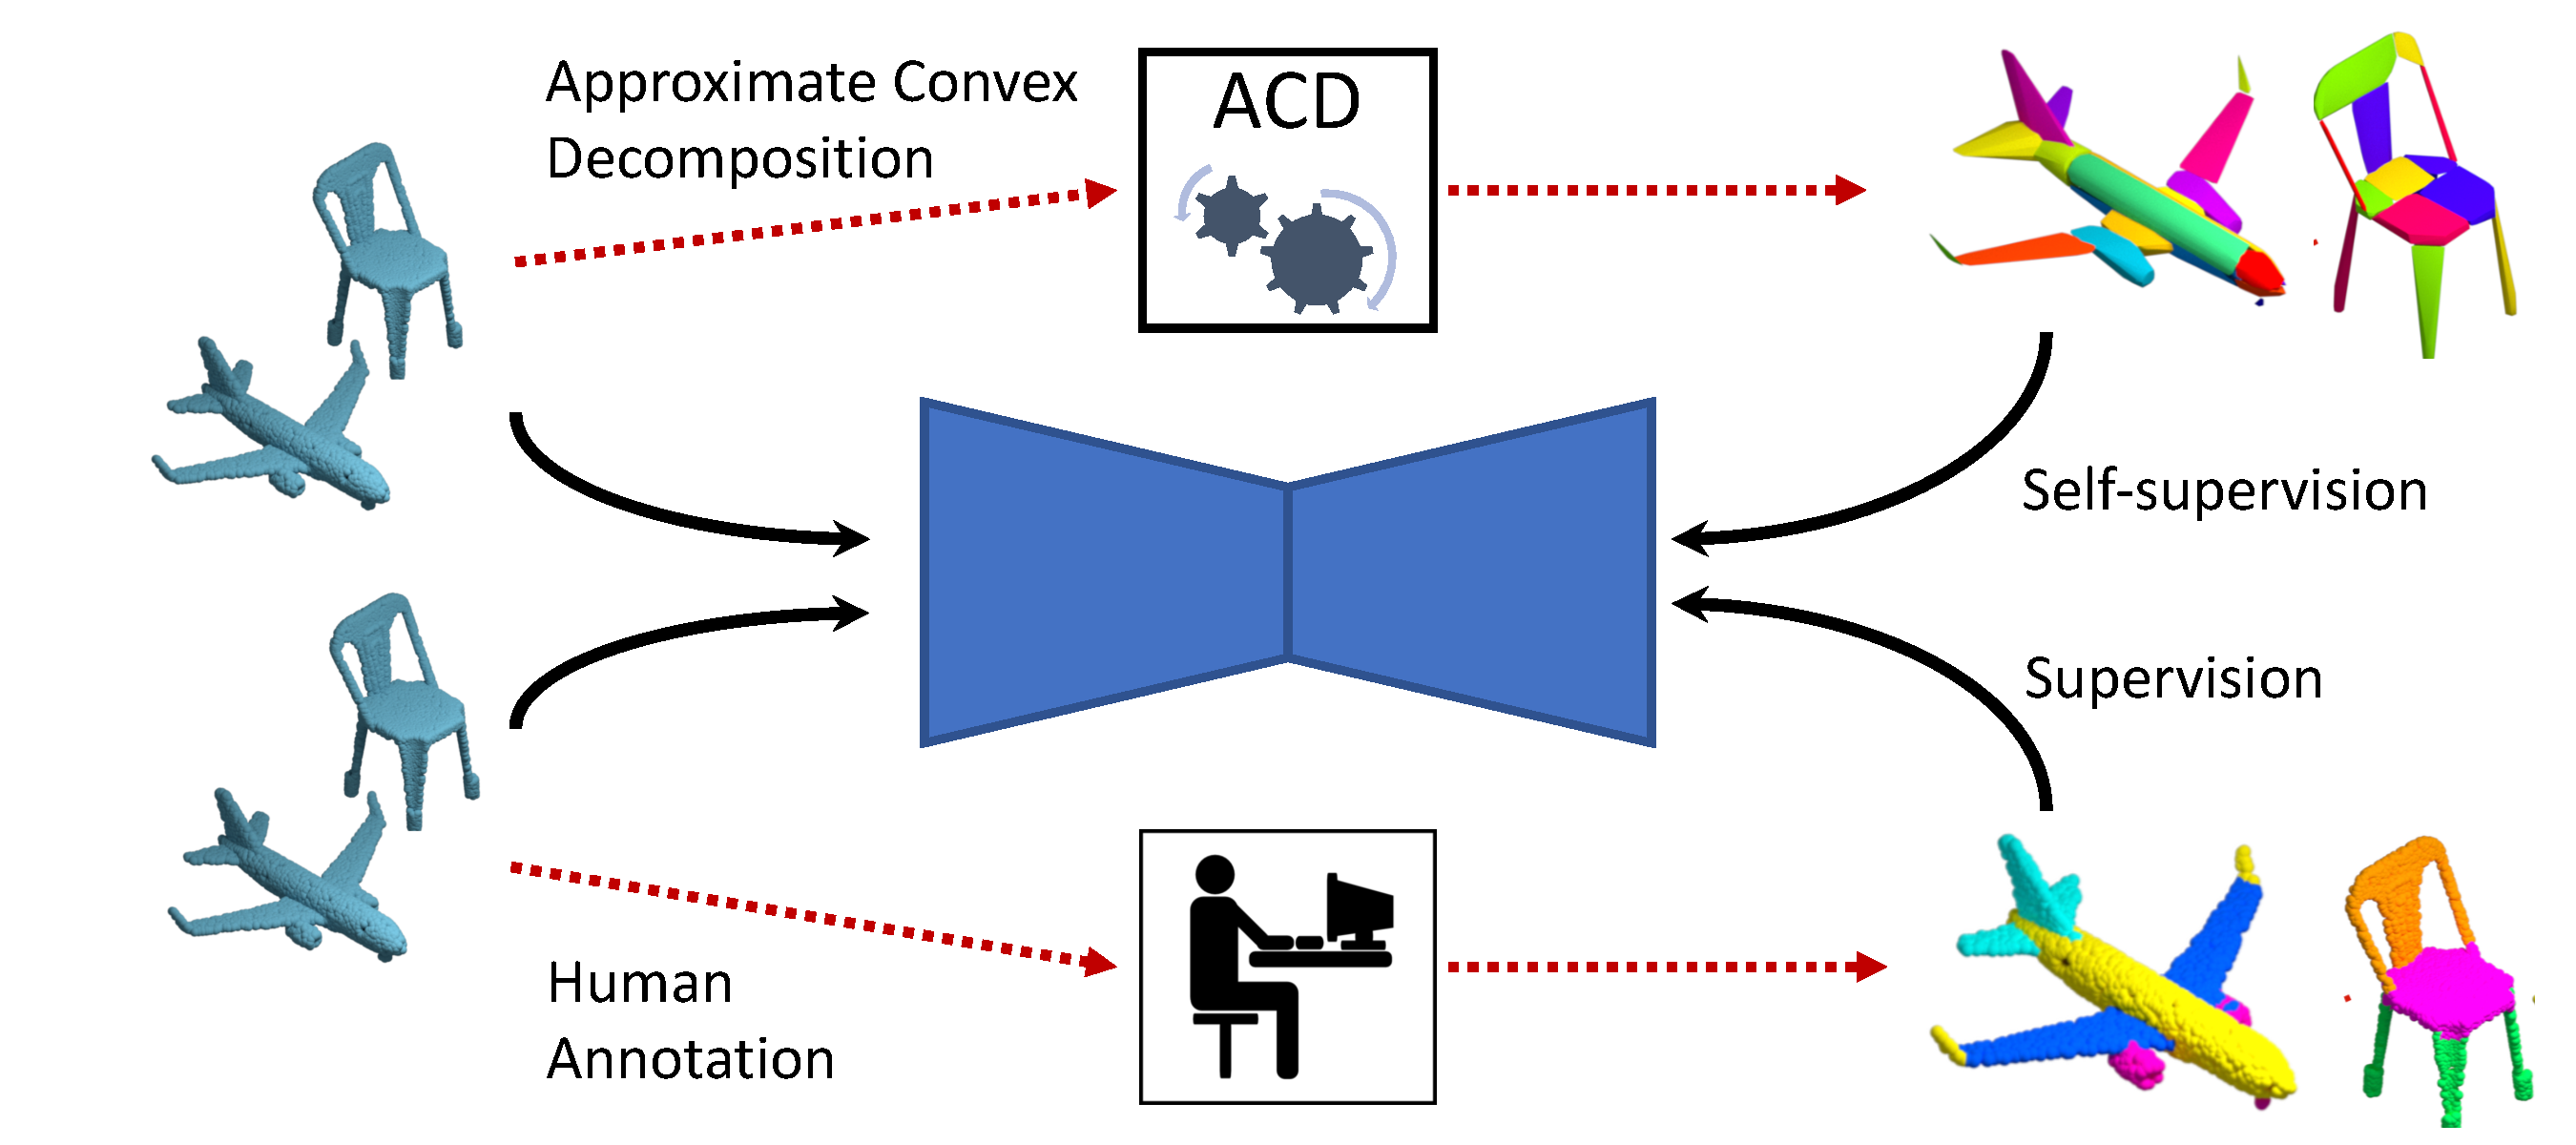
\includegraphics[width=\linewidth]{acd/imgs/visual-summary.pdf}
    \caption{\small{Overview of our method v.s. a fully-supervised approach. \textit{\textbf{Top:}} Approximate Convex Decomposition (ACD) can be applied on a large repository of unlabeled point clouds, yielding a \textit{self-supervised} training signal for the neural network without involving any human annotators. \textit{\textbf{Bottom:}} the usual \textit{fully-supervised} setting, where human annotators label the semantic parts of point clouds, which are then used as supervision for the neural network. The unsupervised ACD task results in the neural network learning useful representations from unlabeled data, significantly improving performance in shape classification and semantic segmentation  when labeled data is scarce or unavailable.}
    }
    % \rui{as the figure is titled `overview of our approach', it looks like the bottom is also part of our approach. Maybe the caption can be changed to `overview of our approach vs. fully supervised approach' or something like that.}}
    % \llcao{Is it possible to show another figure comparing the effects of decomposing via ACD and exact convex decomposition? That may help the reviews understand what ACD is like }}
    \label{fig:vis_summary}
\end{figure}

The performance of current deep neural network models on tasks such as classification and semantic segmentation of point cloud data is limited 
by the
amount of high quality labeled data available for training the networks. 
Since in many situations collecting high quality annotations on point 
cloud data is time consuming and incurs a high cost, there has  
been increasing efforts in circumventing this problem by training 
the neural networks on noisy or weakly labeled datasets~\cite{SharmaPEN},
or training  in completely unsupervised ways~\cite{hassani2019unsupervised,mrt18,yang2018foldingnet,yang2019pointflow,chen2019bae}. 

% In this work, we propose
% to learn local and global
% shape representations using a self-supervision task in which a neural
% network is trained to decompose an input point cloud into 
% \textit{approximate convex parts}. These shape representations are shown 
% to be useful in few-shot semantic segmentation and classification tasks.
%
A ubiquitous technique in training deep networks is to train the
network on one task to initialize its parameters and learn generically
useful features, and then fine-tune the network on the final
task. In particular, there has been great interest in so-called {\em
  self-supervised} tasks for initialization. These tasks, which do not
require any human annotations, allow the network to be initialized by
using various techniques to generate labels automatically, \ie, in a
self-supervised manner -- \eg tasks such as clustering, solving jigsaw
puzzles, and colorization. 
% In this work, we propose to \rui{missing something} 
There have been
a few recent attempts to come up with similar tasks that help with 3D
data~\cite{hassani2019unsupervised,chen2019bae}.  The overarching question
here is \textit{``what makes for a good self-supervision task?''} --
what are the useful inductive biases that our model learns from
solving such a task that is beneficial to the actual downstream target
task we are interested in solving.  
% For 3D shapes, the downstream task
% is typically shape classification or part segmentation.

We propose using a classical shape decomposition method, Approximate Convex Decomposition (ACD), as the
self-supervisory signal to train neural networks built to process 3D
data. We posit that being able to decompose a shape into geometrically
simple constituent parts provides an excellent self-supervisory learning
signal for such purposes. As shown in the Figure
\ref{fig:samples-of-acds}, ACD decomposes shapes into segments that
roughly align with instances of different parts, \eg two wings
of an airplane are decomposed into two separate approximately convex
parts. Many man-made shapes are influenced by physical and geometric 
constraints. 
Convex parts tend to be easily manufactured, and are strong and aerodynamic, thus fulfilling the above
requirements. 
However, strictly convex decomposition often leads to highly
over-segmented shapes.  
For that reason, we chose \textit{approximate}
convex decomposition, which we show benefits a number
of learning tasks.

Our approach is illustrated in Figure~\ref{fig:vis_summary}.  The main
idea is to automatically generate training data by decomposing
unlabeled 3D shapes into convex components.  Since ACD relies solely
on geometric information to perform its decomposition, the process
does not require any human intervention.  From the model perspective,
we formulate ACD as a metric learning problem on point embedding and
train the model using a contrastive
loss~\cite{hadsell2006dimensionality,chopra2005learning}.  
We demonstrate the
effectiveness of our approach on standard 3D shape classification and
segmentation benchmarks.  In classification, we show that the
representation learned from performing shape decomposition leads to
features that achieve state-of-the-art performance on
ModelNet40~\cite{wu20153d} unsupervised shape classification ($\mathbf{89.8\%}$).  For
few-shot part segmentation on ShapeNet~\cite{Chang2015ShapeNetAI}, our
model outperforms the state-of-the-art by \textbf{7.5\%} mIoU when
using 1\% of the available labeled training data.  Moreover, differently from
other unsupervised approaches, our method can be applied to any of the
well-known neural network backbones for point cloud processing.
Finally, we provide thorough experimental analysis and visualizations
demonstrating the role of the ACD self-supervision on the
representations learned by neural networks.
